%*******************************************************************************
%****************************** Second Chapter *********************************
%*******************************************************************************

\chapter{The execution semantic of Stream Processing in Flink (10 pages)}

\ifpdf
    \graphicspath{{Chapter3/Figs/Raster/}{Chapter3/Figs/PDF/}{Chapter3/Figs/}}
\else
    \graphicspath{{Chapter3/Figs/Vector/}{Chapter3/Figs/}}
\fi

\section{Heterogeneity}
Since the first commercial project of Complex Event Processing launched by Bell Labs in 1998 with its "Sunrise Project", we have seen the fast growing of many stream processing frameworks. However, there is a huge degree of heterogeneity across these frameworks in various forms\citep{Dindar:2013}

\begin{enumerate}

	\item Syntax: Although the ISO/IEC 9075 is published standard to defines the complete syntax and operations in SQL language as a whole, there is no standard language for stream processing. Different stream processing engines use different syntax to depict the same function. For example,every 5 seconds, a window captures all event last 10 seconds. 
	\begin{verbatim}
	CQL: 	[RANGE 10 seconds SLIDE 5 second ] 
	Flink: 	[SIZE 10 sec EVERY 5 sec]
	\end{verbatim}
	
	\item Capability heterogeneity:
	Those engines also provide different set of query types and operations based on which functions they are capable of. For examples, \textit{Streambase} support pattern matching on stream, whereas STREAM does not.
	
	\item Execution Model: Below the language level, hidden from application layers, each stream processing engine has its own underlying execution model. With the same data stream but different model produce different output which varies based on the differences on tuple ordering,  window construction, evaluation and so on. We are going to focus on the differences between several existing execution models below.
	
	
\end{enumerate}
 
We have learned that there are at least three different execution models:
\begin{itemize}
	\item \textbf{Time-driven} execution model, followed by CQL, Oracle CEP. In the model, each tuple have a timestamp. Timestamp induces the total order of tuples on stream, but not a strict total order. Or more specifically, there is no ordering between tuples with identical timestamps. These tuples are consider as simultaneous tuples. It is problematic when we select a window of last 10 tuples but more than 10 simultaneous tuples arrived at a given time instant. In this case, there is no different between those tuples, the system will select only 10 out of all in a non-deterministic way.
	
Assuming that we has stream $\mathbb{S}$
	\begin{equation}
			\mathbb{S}(value, t_{app}) = (1,1),(10,2),(20,2), (100,3)
	\end{equation}
	

	
Consider a query which continuously recall the last arrival tuple i.e., we select tuple-based window with size of 1 tuple. In the time-based execution model,  the state of a window changes as timestamp progress. Window get re-evaluated only when timestamp change. At $t=1$ or $t=3$, there is only 1 arrival tuple, new 1-tuple-size window will open , pick the tuple then close. Thus the stream derives window $W_1: \{(1,1)\}$ and $W_3: \{(100,3)\}$. On other hand, at $t=2$, there are 3 new arrival tuples. New window $W_2$ opens and be able to pick 1 tuple only. Since these 3 tuples arrive simultaneously, they will have the same timestamp and thus no any temporal differences between them.
Engine randomly pick one of them for window $W_2$. In short, window $W_2$ contains one of following options: $(10,2)$ or $(20,2)$. The derived stream will be one of the streams:
\begin{verbatim}
(1,1),(10,2), (100,3) or (1,1),(20,2), (100,3)
\end{verbatim}

\begin{figure}[htbp!] 
\centering    
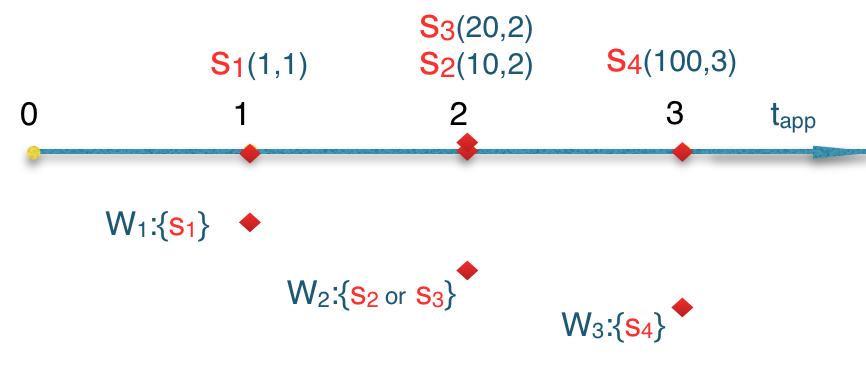
\includegraphics[width=0.5\textwidth]{time-driven}
\caption{time-driven}
\label{fig:time-driven}
\end{figure}
	
	\item \textbf{Tuple-driven} execution model, followed by StreamBase, Apache Flink. In this model, tuples may have an application timestamp attribute on its schema. Some of timestamp values might be identical but tuples themselves are completely distinguished in stream. There exists a strict total order in stream based on their arrival order. 
	
	There are several ways to represent tuple order in stream. StreamBase system assigns an incremental internal rank to tuples to arriving tuples. It ensures that the tuple with lower rank with be processed before tuples with higher rank. In Apache Flink, we implicitly use system timestamp   $t_{sys}$ at which system receives the tuple. Since system timestamp are strictly totally ordered, it is simply suitable for Flink execution model. Several other works propose to use tuple Id \citep{Dindar:2013} or a physical identifier\citep{Petit:2010} instead. 	
	
	In tuple-drive execution model, each tuple arrival cause a system to react, instead of each application timestamp progress. In previous example, tuple $(10,2)$ and $(20,2)$ has the same application timestamp but system will open a new 1-tuple-size window for each of them. Therefore,assuming that tuple $(10,2)$ arrives before tuple $(20,2)$, the derived stream will be exact as 
	\begin{verbatim}
		(1,1),(10,2),(20,2), (100,3)
	\end{verbatim}
	
	\begin{figure}[htbp!] 
\centering    
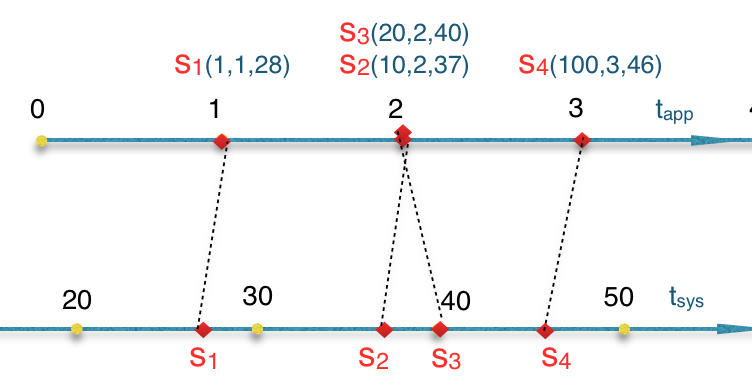
\includegraphics[width=0.5\textwidth]{tuple-driven}
\caption{tuple-driven}
\label{fig:tuple-driven}
\end{figure}
	
	\item \textbf{Batch-driven} execution model, followed by Coral8, mentioned in SECRET\citep{Botan:2010} descriptive model
\end{itemize}. In this model, each tuple is assigned an batch-id. Every tuple which belong to a batch must have the same timestamp, but 2 separate tuple with the identical timestamp may belong to two different batches. As we can see, batch-driven model is in between of tuple-driven and time-driven model (Figure~\ref{fig:executionModel}). Assuming that at a given application timestamp $\tau$, the system receives 5 tuples ${<v_1,\tau>,<v_2,\tau>,<v_3,\tau>,<v_4,\tau>,<v_5,\tau>}$. Time-driven model treats them as simultaneous tuples with no difference. Tuple-driven considers them as 5 concrete tuples in strict order. And batch-driven model may divide them into 2 batches $\{<v_1,\tau>,<v_2,\tau>,<v_3,\tau>\}$, $\{<v_4,\tau>,<v_5,\tau>\}$ depending on window specification.


	\begin{figure}[htbp!] 
\centering    
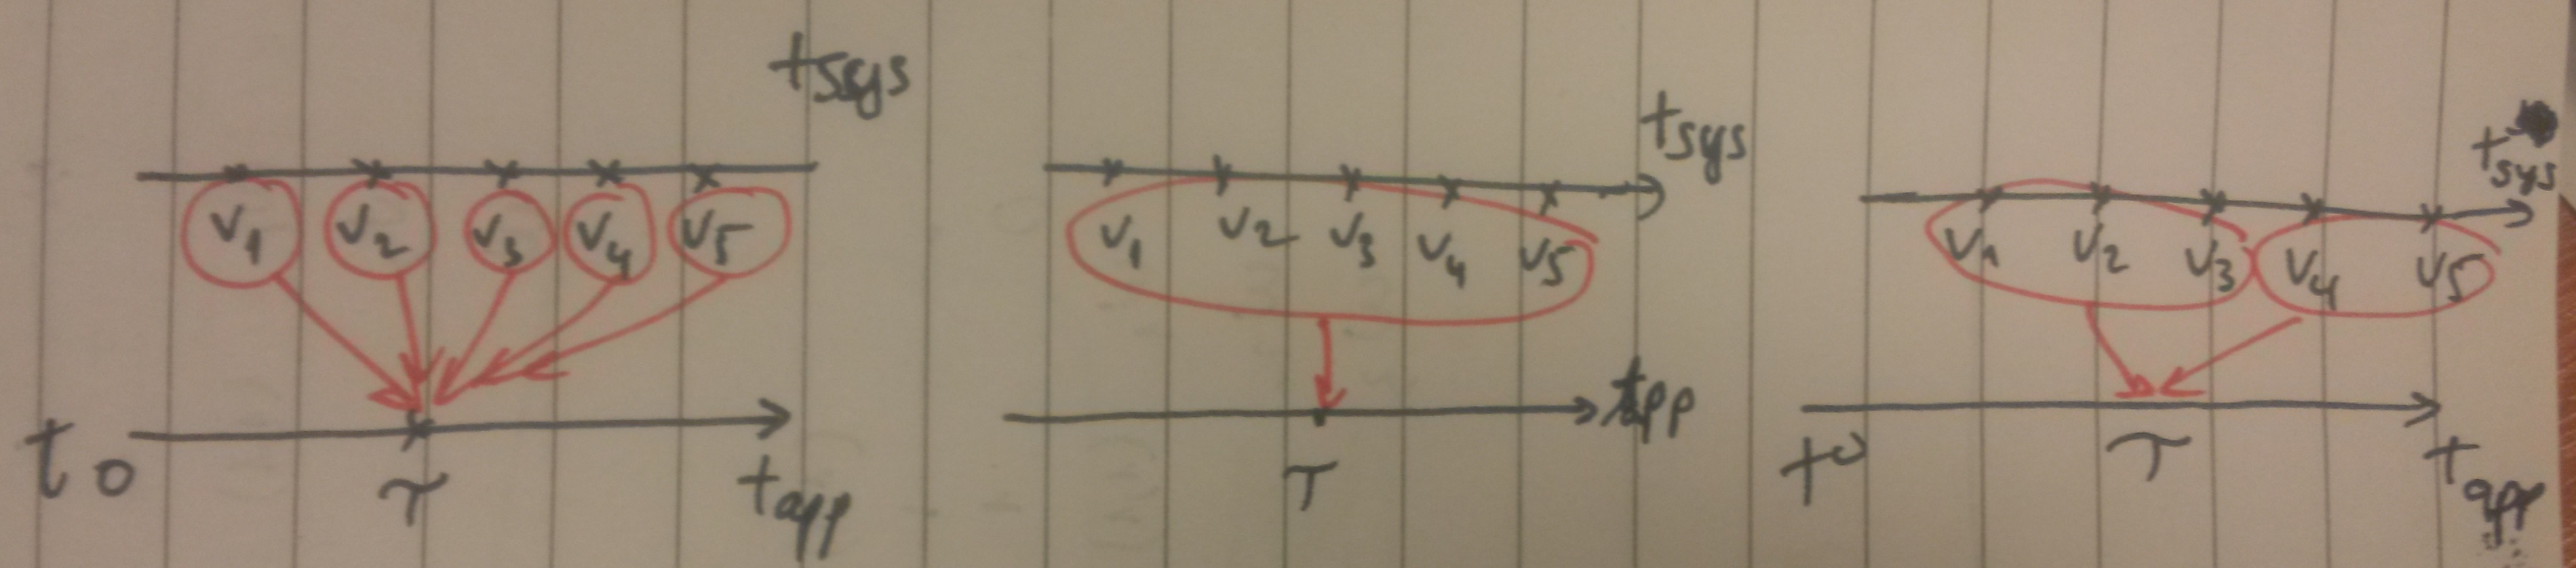
\includegraphics[width=1\textwidth]{executionModel}
\caption{executionModel}
\label{fig:executionModel}
\end{figure}


We extends the examples \citep{Dindar:2013} with Flink implementation in order to demonstrate that system with different execution model may produce different output , even with the same input and query. 
\begin{enumerate}

\item Example 1: differences in window constructions
Given \textit{Instream} stream with schema $S(time, value)$. Consider a query which continuously computes the average value of tuples in a time-based tumbling window of size 3.
\begin{align*}
Instream(time,value) &= \{(10,10),(11,20),(12,30),(13,40),(14,50),\\
&\qquad (15,60),(16,70),...\} \\
Oracle\, CEP\, (avg)		&= \{(20), (50),...\} \\
Flink\, (avg)			&= \{(15), (40),...\} \\
\end{align*}

Obviously, Oracle CEP constructs the first window with first 3 tuples whereas Flink picks first 2 tuples only. The second window , they both take next 3 tuples. We implement the test on Flink with default configuration, however we are able to customize the upper bound of the first window ($startTime = 12$)so that it produces the same result as Oracle CEP.


\item Example 2: differences in window evaluations

Consider a query which continuously computer the average value of tuples over last 5 second once every 1 second (time-based window of size 5s that slides by 1s)

\begin{align*}
Instream(time,value) 	&= \{(30,10),(31,20),(36,30),...\} \\
Oracle\, CEP\, (avg)		&= \{(10), (15),(20),...\} \\
Flink\, (avg)			&= \{(10), (15), (15), (15), (15), (20),...\}\\
Coral8\, (avg)			&= \{(10), (15),(20),...\}			
\end{align*}

Flink produced a different result than Oracle and Coral8.
In Oracle and Coral8, a new window is emitted for invoking the average operator only when the window content's change; whereas in Flink, it emits a new window every second as the sliding progress , even if the content does not change. The state of window is depicted on Figure ~\ref{fig:winEvaluation}
\begin{figure}[htbp!] 
\centering    
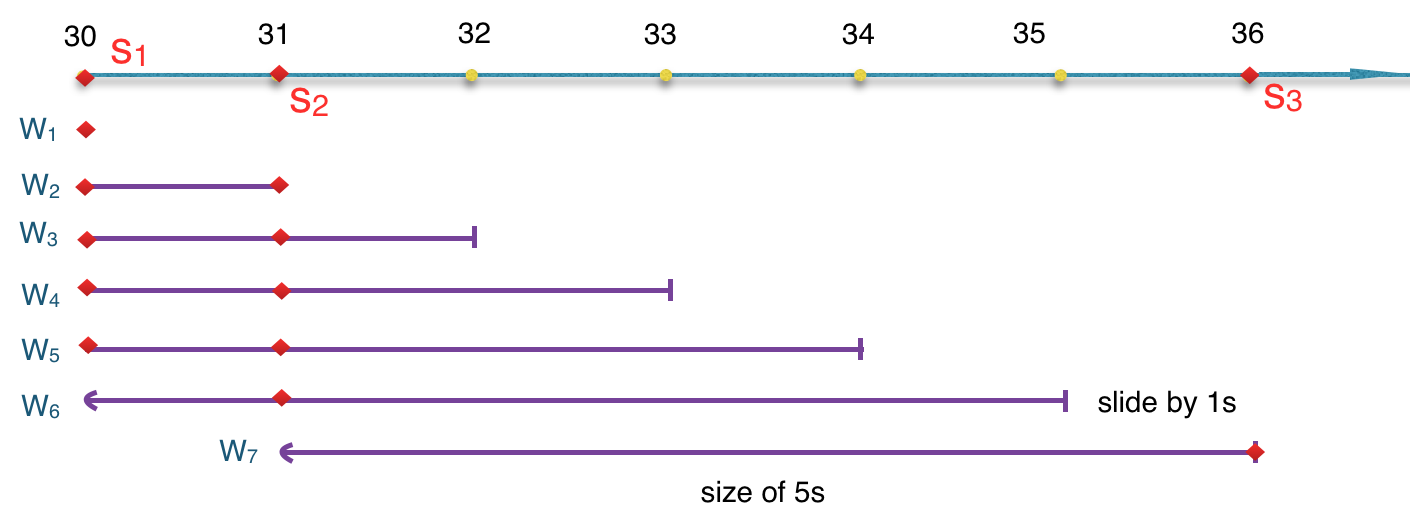
\includegraphics[width=0.7\textwidth]{winEvaluation}
\caption{Window State}
\label{fig:winEvaluation}
\end{figure}

Remember that window closes at upper boundary and opens at lower boundary so that in window $W_6$ cover from $t=35$ to right after $t=30$ will exclude tuple $(30,10)$. Similarly, $W_7$ excludes tuple $(31,20)$


\item Example 3: differences in processing granularity

Consider a query which computes the average value of tuples over a tuple-based tumbling window of size 1 tuple.
\begin{align*}
Instream(time,value) 	&= \{(10,10),(10,20),\\
						&\quad (11,30),\\
						&\quad (12,40),(12,50),(12,60),(12,70),\\
						&\quad (13,80),...\} \\
Oracle\, CEP\, (avg)		&= \{(20), (30),(70),(80)...\} \\
Flink\, (avg)			&= \{(10), (20), (30), (40), (50), (60),(70),(80)...\}\\
Coral8\, (avg)			&= \{(10), (20), (30), (40), (50), (60),(70),(80)...\}
\end{align*}

Oracle CEP implements time-based execution model so that it reacts to each application timestamp. If there are multiple simultaneously tuple arrive, it will pick one of them non-deterministically to construct the window , since window size is 1. In other hand, Flink and Coral8 react to every tuple arrival so that they emit new 1-tuple-size tumbling window for every tuple.

\end{enumerate}

tuple: each tuple arrival cause a system to react
time: the progress of tapp cause a system to react
batch:  where either a new batch arrival or the progress of tapp cause a system to react

\section{Policy-based Window Semantics}


Flink constructs windows based on parameters in specification. Currently Flink does not support Predicate Window so that two of most critical parameters are to notify when system should trigger new windows (indicating the lower bound of window) and when system must end the window (indicating the upper bound of window) and emit it to window stream. For that purpose, Flink implements a mechanism called \textit{"Policy-based windowing"}. It is a highly flexible way to specify stream descretization. It has two independent policies corresponding to open and close window: Trigger and Eviction Policy.
To demonstrate the concepts of two policies, let's consider the scenario with \textit{StockTick} stream: check every 10 minutes the total transaction volume of all transaction last 30 minutes. In other words, in every 10 minutes create a new window to cover all the transactions in last 30 minutes. The syntax in Fink:

\begin{verbatim}
StockTick.window(Time.of(30, MINUTES))
		 .every(Time.of(10, MINUTES)).sum(Quantity)
\end{verbatim}

\begin{enumerate}

\item Eviction Policy: define the length of a window. The length is passed in to \textit{window(...)} function. It could be the time interval, number of tuples and delta function with threshold (in case of delta window).
We formalize the concept of window due to its size

\begin{defi}
A time-based window $W_{t} = (l,u,\omega)$ over a stream $S$ is a finite subset of  $\mathbb{S}$ containing all data elements $s \in \mathbb{S}$ where $l , u, \omega \in \mathbb{T}$ and$l < s.t \leq u$. The length of window in time unit is $\omega = u-l$
\end{defi}
Notice that in a time-based window, $s.t$ can be tuple's application or system timestamp depending on query. There are maybe many simultaneous tuple with identical $t_{app}$. However, there is at least one arriving tuple at a given $t_{sys}$. The second point is that $W_t$ open at $t = l$, it does not include tuple at this time instant.

\begin{defi}
A count-based window $W_{c} = (l,u,n)$ over a stream $S$ is also a finite subset of  $\mathbb{S}$ containing all data elements $s \in \mathbb{S}$ where $l,u \in \mathbb{T}$, $\omega \in \mathbb{N}$ and $l \leq s.t_{sys} \leq u$. The length of window is the number of tuples in interval time $(l, u]$, i.e., $|n {s \in \mathbb{S}(t_{sys}): l < s.t_{sys} \leq u}|$
\end{defi}
The count-based window $W_{c}$ is independent from application timestamp $t_{app}$. It is related to system timstamp $t_{sys}$ which indicate tuple's order in stream. 


\item Trigger Policy: In general, it defines window slide or the distance between 2 consecutive windows. On above example , trigger policy states that from beginning, system must trigger a new window every 10 minutes. No other window would be triggered within this 10 minutes. 

Suppose that we have 2 consecutive windows $W^1 = (l_1, u_1, \_)$ and $W^2 = (l_2, u_2, \_)$  where $l_1 < l_2$. There is no window $W^1 = (l_3, u_3, \_)$ such that $l_1< l_3 < l_2$.
\begin{itemize}

\item If $W_1$ and $W_2$ are time-based windows, a slide $\beta_{t} = u_2 - u_1$.  
\item If $W_1$ and $W_2$ are count-based windows, a slide $\beta_{c} = |{s \in \mathbb{S}(t_{sys}): u_1 < s.t_{sys} \leq u_2}| $ 

\end{itemize}

\end{enumerate}

If the correlation between window size and slide size  conforms to the movement type of windows.
\begin{itemize}
\item Sliding window: $\omega > \beta$ or $n > e$
\item Tumbling window: $\omega = \beta$ or $n = e$
\item Jumping window: $\omega < \beta$ or $n < e$
\end{itemize}

However, Flink allow to mix between time-based trigger policy with count-based eviction policy and vice versa. For example,
calculate sum of quantities of last 100 transactions every 1 hour.
\begin{verbatim}
StockTick.window(Count.of(100))
		 .every(Time.of(1, HOURS)).sum(Quantity)
\end{verbatim}

\section{The execution semantic}

%\begin{verbatim}
%
%		boolean isTriggered = false;
%
%		if (triggerPolicy.notifyTrigger(input)) {
%			emitWindow();
%			isTriggered = true;
%		}
%
%		evict(input, isTriggered);
%
%		collector.collect(windowEvent.setElement(input));
%		bufferSize++;
%
%\end{verbatim}

Window Buffer \textit{wb} is a linking list contain tuple with composite type $IN$



\begin{equation}
	t = 
	\begin{cases}
		t_{sys} \qquad if\,t_{app} = None\\
		   \\
		t_{app} \qquad\qquad\qquad otherwise
	\end{cases}
\end{equation}

$size_{t}(wb) = wb.last.t - wb.first.t$

$size_c(wb) = wb.length()$


\begin{algorithm}
\caption{Process new arrived tuple}
\label{algorithm:processNewTuple}
The first step, before processing a new arrived tuple, check if a current window buffer should be emit. If yes, copy the current window buffer to a window object and put to Windowed Stream. The second step, calculating which tuples should be evicted if the current window buffer appends new arrived tuple. There are two separate case for time-based and tuple-based window. The third step, evicting those tuples and appending new arrived tuple.


\algrenewcommand\algorithmicfunction{\textbf{class}}
\algrenewcommand\algorithmicprocedure{\textbf{method}}
  \begin{algorithmic}[1]
  	\Require {$wb$: the current window buffer}
  	
  			{$\omega_t$: size of window in time interval }
  			
  			{$\omega_c$: size of window in tuple count }
    %\Function{Mapper}{}
    \Procedure{processNewTuple}{$\textrm{newTuple }: IN$}
    
    \If{$\textsc{notifyTrigger}(newTuple)$} \Comment{ trigger new window if full}
    		\State $\textrm{window} \gets \textrm{wb}$
    		\State $\textsc{Emit}(\textrm{window})$ \Comment {emit to Windowed stream}
    \EndIf
    
    \If{$\textrm{window is time-based}$}
    		\State $ evict_t \gets size_t (\textrm{wb.append(newTuple)}) - \omega_t$
    
    		\If{$evict_t > 0$} \Comment {remove old tuples}
    			\State $ \textrm{lastEvictedTimestamp} \gets wb.first.t + evict_t - 1$
    			\ForAll{element $e$ in window buffer $wb$}
    				\If {$e.t \leq \textrm{lastEvictedTimestamp}$}
    					\State $wb.remove(e)$
    				\EndIf
    			\EndFor
    		\EndIf
    \Else \Comment{window is count-based}
    		\State $evict_c \gets size_c(\textrm{wb.append(newTuple)}) - \omega_c$
    		\If{$evict_c > 0$} \Comment {remove old tuples}
    			\For {$i \gets 1, evict_c$}
    				\State $wb.removeFirst()$
    			\EndFor
    		\EndIf
    \EndIf
    
   	\State $wb \gets wb.append(newTuple)$ \Comment {add new tuple to current window buffer}
    
    
    \EndProcedure
    %\EndFunction
  \end{algorithmic}
  




\end{algorithm}


\begin{algorithm}
\caption{Trigger a new window if full }
\label{algorithm:notifyTrigger}
When a new tuple has arrive, system check whether the current window buffer reached the point where distance of 2 windows is equal to slide size or not. The new tuple is not really appended to buffer, use it for qualifying purpose only.
\begin{algorithmic}[1]
  	\Require {$\beta_c$: count-based slide size}
  			{$\beta_t$: time-based slide size }
  			{$lastUpperBound$: upper boundaries of previous window}
    %\Function{Mapper}{}
    \Procedure{notifyTrigger}{$\textrm{newTuple }: IN$}
    
   
    
    \If{$\textrm{window is time-based}$}
    		\If{$\textrm{size_t} (\textrm{wb.append(newTuple)}) > \beta_t$}
    			\State $\textrm{lastUpperBound} \gets \textrm{newTuple.t}$
    			\State $\textrm{return true}$
    		\Else
    			\State$\textrm{return false}$
    		\EndIf
    
    \Else \Comment{window is count-based}
    		\If{$\textrm{counter} \geqslant \beta_c $}
    			\State $\textrm{counter} \gets 1$
    			\State $\textrm{return true}$
    		\Else
    			\State $\textrm{counter} \gets \textrm{counter} + 1$
    			\State $\textrm{return false}$
    		\EndIf
    	\EndIf
    
    
    \EndProcedure
    %\EndFunction
  \end{algorithmic}
\end{algorithm}

